\documentclass[conference]{IEEEtran}
\usepackage[T1]{fontenc}
\usepackage[utf8]{inputenc}
\usepackage{amsmath}
\usepackage{booktabs}
\usepackage{array}
\usepackage{pgfplots}
\pgfplotsset{compat=1.18}
\usepackage[hidelinks]{hyperref}
\usepackage{microtype}

\begin{document}

\title{Small, Licence-Clean 4x Photo Upscalers for the Apple Neural Engine, and What Frame-by-Frame Video Does to
Them}
\author{\IEEEauthorblockN{Hermes Reisner}
\IEEEauthorblockA{\url{https://github.com/HerRei/localsr-models}}}
\maketitle

\begin{abstract}
This report describes two 4x photo super-resolution models I trained for the LocalSR app: Photo S (0.62M parameters)
and Photo M (2.03M). The training data is a CC0 photo collection, and both models run with every operation of their
Core ML export on the Apple Neural Engine, at 188 and 485\,ms per input megapixel on an M1 Pro. On a sealed DIV2K
hold-out that was scored once, at each file's own operating point, Photo S beats the SPAN model it is meant to replace
on LPIPS and DISTS at 1.4\,dB higher PSNR. Photo M shows no clear difference to a 7.4M-parameter RealPLKSR model on
LPIPS and DISTS, at 2.6\,dB higher PSNR. The report has three parts. The first is the evaluation: paired bootstrap
intervals over photos, seed replicates, and comparisons at matched fidelity on the development set. The second is a
blur diagnosis: the real-camera test sets are blurrier than what my first models restore, and a lens-blur regime in
the training degradations improves RealSR clearly in two seeds, while noisy soft input stays weak. The third is
frame-by-frame video: the GAN texture of these models flickers 1.5 to 1.9 times as much as their L1 parents, a cheap
temporal blend helps on still shots, and a consistency fine-tune trades sharpness for less flicker without passing
the rule I set before training. The weights are released under CC BY 4.0, the code under MIT.
\end{abstract}

\section{Introduction}

I wanted models that run on the NPU, so I can upscale things while still using my computer. I also wanted to
find out what these NPUs can really do, because there is little practical experience with super-resolution on
them. On Apple Silicon the NPU is
the Neural Engine, and the models are made for the Quick and Best presets of LocalSR, a free app that upscales
photos and videos on the user's own machine.

I set three constraints for the models:
\begin{itemize}
\item \textbf{Licence-clean data.} Every training image comes from a collection its publisher releases as CC0, so the
  weights can be shared under a permissive licence.
\item \textbf{The Neural Engine.} It only runs a narrow set of operations well. Therefore the network uses nothing but
  plain convolutions, ReLU, additions, and pixel shuffle.
\item \textbf{Decided by measurement.} Small models differ by small margins, and image-quality judges often disagree
  about them. Most decisions in this project used a rule written before the result. Where a model did not pass its
  rule, I say so.
\end{itemize}

\section{Related Work}

Real-world super-resolution usually trains on synthetic degradations. BSRGAN~\cite{bsrgan} randomises blur, noise,
resizing, and JPEG, and Real-ESRGAN~\cite{realesrgan} adds a second-order pipeline. Efficient models such as
SPAN~\cite{span} aim at speed with few parameters. My network follows the PULSE layout specified by Philip
Hofmann~\cite{pulse}, with a fixed Magic Kernel Sharp~\cite{mks} upscale as its base. The losses combine pixel terms
and MS-SSIM~\cite{msssim} with DINOv2~\cite{dinov2} features, a sliced Wasserstein term on those features in the
spirit of texture synthesis~\cite{sliced}, and a PatchGAN~\cite{pix2pix} with feature matching~\cite{improvedgan}. The
judges are LPIPS~\cite{lpips}, DISTS~\cite{dists}, A-FINE~\cite{afine}, and TOPIQ~\cite{topiq}, on the
RealSR~\cite{realsr} and DRealSR~\cite{drealsr} crops published with StableSR~\cite{stablesr}, and on
DIV2K~\cite{div2k} for the hold-out. A large user study found that LPIPS and DISTS can fail on fine-grained
comparisons of super-resolution results~\cite{su}, which matters here because the differences are small. Temporal
consistency of per-frame processing has been handled with post-hoc networks~\cite{lai} and with temporal losses in
video GANs~\cite{tecogan}. The video part of this report measures the simplest versions of both ideas on tiny models.
It does not propose a new method.

\section{Models and Training}

\subsection{Network}
PULSE maps the input through a $3\times3$ stem convolution to $d$ channels, $n$ residual blocks of two bias-free
$3\times3$ convolutions with a ReLU between them, a global residual, and a $3\times3$ head to $3\cdot16$ channels
with pixel shuffle. The head's output is added to a fixed Magic Kernel Sharp $4\times$ upscale of the input, so the
network only learns a residual. Photo S uses $d=64$, $n=8$ (619{,}248 parameters), Photo M uses $d=96$, $n=12$
(2{,}034{,}768). The released files are named after scale, purpose, network, and size:
\texttt{4xLocalSRPhoto\_PULSE-64x8} and \texttt{4xLocalSRPhoto\_PULSE-96x12}. In the Core ML export on an M1 Pro every operation runs on the Neural Engine (40 of 40 for Photo S, 56
of 56 for Photo M, fp16).

\subsection{Data}
All training images come from lucid-cc0-v2-hc~\cite{lucid}, photographs from pxhere that the collection's publisher
releases as CC0, as 256 and 512\,px tiles (193{,}262 tiles of 1{,}397 source photos in the 256\,px set). Validation
tiles are split by source photo. According to the export cards, both released models descend only from my own runs on
this data. No third-party weights are in their lineage. DINOv2 (Apache-2.0) is used as a loss network during
training and is not part of the weights.

\subsection{Degradations}
The low-resolution inputs come from my own phone-photo pipeline. It mixes capture regimes with Gaussian and motion
blur, digital zoom, several resampling kernels, sensor noise with a demosaic-like spatial correlation, noise
reduction, sharpening, and JPEG, WebP, HEIC, or AVIF. HEIC and AVIF draws, about a third of all draws, come from a
pre-baked set made with an earlier version of the pipeline. With probability 0.5 the high-resolution target is first
downscaled by 1.25 to 2$\times$ to reduce its own noise. Photo M adds a \emph{lens} regime (Section~\ref{sec:blur}): half
of the daylight, night, and zoom draws get a near-isotropic blur with $\sigma$ between 1.4 and 3.6 HR pixels, without
noise reduction or sharpening.

\subsection{Losses and Phases}
Each model is trained in two phases on 192\,px crops, batch 32, fp16, with an EMA of the weights (decay 0.999). The L1
phase uses an L1 loss only. The GAN phase (80k updates, learning rate $5\cdot10^{-5}$) uses L1 1.0, colour 0.05,
MS-SSIM 0.25, discriminator feature matching 0.1, L1 on DINOv2 ViT-S/14 features of blocks 3, 6, and 9 0.1, a sliced
Wasserstein term on the same tokens 0.1, and the adversarial term 0.03, ramped in over 5k updates. Each model
warm-starts from earlier runs of my own.

\subsection{Released Files}
The released files are blends of the two phases' weights. The blend factor sets the operating point. I fixed it at a
web-copy PSNR-Y of 28.4\,dB, a development point I chose by eye on eight of the 166 web copies. Photo S uses the GAN
body and a head of 60\,\% GAN and 40\,\% L1 weights. Photo M uses the GAN weights. Before release the head is adjusted by
a small ridge regression so that its 16 sub-pixel phases respond equally on flat colour areas (\emph{phase
flattening}). This removes a faint 4\,px checkerboard that GAN training leaves. Two guards check flat-region speckle
and the remaining phase pattern.

\section{Evaluation}

\begin{itemize}
\item \textbf{Web copies} (development): 166 of my own photographs, downscaled to 512\,px on the long side and saved
  as JPEG 85 with 4:2:0 chroma, against a 4$\times$ reference.
\item \textbf{RealSR and DRealSR} (real cameras): the 512\,px centre crops of StableSR, 100 and 93 images with
  128\,px LR. They were also used during development.
\item \textbf{Sealed hold-out}: the 100 DIV2K validation photos through the same web-copy pipeline (99 pass the
  1{,}000\,px minimum). It was built before the final models existed and scored once, in one final run with six files.
  Some third-party models may have trained on DIV2K data.
\item \textbf{Judges}: PSNR-Y and SSIM-Y for fidelity, LPIPS-Alex, LPIPS-VGG, and DISTS as one family of
  deep-feature distances, A-FINE as an independent full-reference judge (on 512\,px tiles for the web copies), and
  TOPIQ as a reported column.
\item \textbf{Statistics}: per-photo paired differences with a 95\,\% percentile bootstrap~\cite{bootstrap} over
  photos (10{,}000 resamples, seed 0), the number of photos where a file is better, and a sign test. A bootstrap over
  photos does not measure the spread between training runs. For that, Photo S has three training seeds and Photo M two.
\end{itemize}

The rule for a camera-oriented Photo M (rule v2) asked for at least 5 points of A-FINE gain on both camera sets with an
interval below zero, a lower fidelity term, TOPIQ not lower, and on the web copies at 28.4\,dB at most $+0.005$
LPIPS and $+0.003$ DISTS. The released Photo M does not pass it (Section~\ref{sec:blur}). I chose it over the same
network without the lens regime as a choice between two finished files.

\section{Results}

\begin{table*}[t]
\centering
\caption{The sealed DIV2K hold-out (99 web copies), scored once. Every file at its own operating point. My files sit
at 28.4\,dB by construction on the development web copies and land there on the hold-out too. The other files are not
matched in fidelity.}
\label{tab:sealed}\small
\begin{tabular}{lrrrrrr}
\toprule
Model & Parameters & PSNR-Y & SSIM-Y & LPIPS & LPIPS-VGG & DISTS \\
\midrule
Photo S & 0.62M & 28.40 & 0.769 & 0.2588 & 0.3734 & 0.1484 \\
\textbf{Photo M} & 2.03M & 28.40 & 0.772 & 0.2450 & 0.3584 & 0.1392 \\
Photo M without lens regime & 2.03M & 28.50 & 0.773 & 0.2402 & 0.3550 & 0.1367 \\
SPAN NomosUni (replaced by Photo S) & 2.24M & 26.97 & 0.746 & 0.2761 & 0.3758 & 0.1591 \\
NomosWebPhoto RealPLKSR (replaced by Photo M) & 7.4M & 25.78 & 0.710 & 0.2485 & 0.3677 & 0.1368 \\
Real-ESRGAN x4plus & 16.7M & 26.22 & 0.742 & 0.2420 & 0.3413 & 0.1281 \\
\bottomrule
\end{tabular}
\end{table*}

\subsection{The Sealed Hold-Out}
Table~\ref{tab:sealed} gives the one scoring of the sealed set. Paired per photo:
\begin{itemize}
\item \textbf{Photo S against SPAN}, the model it is meant to replace: LPIPS $-0.017$ [$-0.022$, $-0.013$], better on
  77 of 99 photos, DISTS $-0.011$ [$-0.016$, $-0.006$], no clear difference on LPIPS-VGG, at $+1.43$\,dB PSNR-Y.
\item \textbf{Photo M against NomosWebPhoto}: no clear difference on LPIPS ($-0.004$ [$-0.012$, $+0.005$]) and DISTS
  ($+0.002$ [$-0.004$, $+0.009$]), LPIPS-VGG $-0.009$ [$-0.016$, $-0.002$], at $+2.62$\,dB PSNR-Y and with about a
  quarter of the parameters.
\item \textbf{Photo M against the same network without the lens regime}: LPIPS $+0.0047$ [$+0.0033$, $+0.0064$] and DISTS
  $+0.0025$ [$+0.0019$, $+0.0031$] at $-0.10$\,dB PSNR-Y. This is the web-photo cost of the lens regime. It has the
  same direction as on the development set ($+0.0059$, $+0.0046$ at matched fidelity) and about half the DISTS cost.
\item \textbf{Real-ESRGAN} has lower LPIPS-VGG and DISTS than both my files and lower LPIPS than Photo S, at 2.2\,dB
  lower PSNR-Y. Against Photo M there is no clear difference on LPIPS.
\end{itemize}

\subsection{Camera Photos}
Table~\ref{tab:camera} shows the real-camera crops. By A-FINE, Photo M is 5.7 points better than Photo S on RealSR and 1.9
on DRealSR. Against the same network without the lens regime it is 5.1 better on RealSR, with no clear difference on
DRealSR. It pays for that with 0.57\,dB (RealSR) and 0.98\,dB (DRealSR) of PSNR-Y. On DRealSR, Photo M is ahead of
NomosWebPhoto by A-FINE and TOPIQ. Real-ESRGAN is ahead on every column of the table.

\begin{table*}[t]
\centering
\caption{Real-camera crops and the web copies. A-FINE on the web copies is the mean over 512\,px tiles. Photo S's A-FINE
is from its released seed, its TOPIQ the mean of three seeds. Across Photo S's three seeds the A-FINE SD is 0.07
(RealSR), 0.01 (DRealSR), and 0.55 (web copies).}
\label{tab:camera}\small
\begin{tabular}{lrrrrr}
\toprule
 & \multicolumn{3}{c}{A-FINE (lower is better)} & \multicolumn{2}{c}{TOPIQ (higher is better)} \\
\cmidrule(lr){2-4}\cmidrule(lr){5-6}
Model (parameters) & RealSR & DRealSR & Web copies & RealSR & DRealSR \\
\midrule
Photo S (0.62M) & 70.82 & 69.10 & 48.46 & 0.340 & 0.337 \\
Photo M without lens regime (2.03M) & 70.17 & 67.75 & 45.95 & 0.349 & 0.346 \\
\textbf{Photo M} (2.03M) & 65.10 & 67.22 & 45.90 & 0.396 & 0.360 \\
NomosWebPhoto RealPLKSR (7.4M) & 58.64 & 70.20 & 34.36 & 0.402 & 0.332 \\
Real-ESRGAN x4plus (16.7M) & 39.45 & 39.98 & 29.01 & 0.416 & 0.388 \\
\bottomrule
\end{tabular}
\end{table*}

On the web copies at 28.4\,dB, Photo M reaches LPIPS 0.2420 and DISTS 0.1361 against Photo S's 0.2555 and 0.1473. Photo S's
three seeds give LPIPS $0.2553 \pm 0.0005$ and DISTS $0.1474 \pm 0.0002$ (mean $\pm$ SD, each file at its own point),
so the gap between Photo S and Photo M is far larger than the spread between Photo S's training runs.

\subsection{Why Small Models Lose on Camera Photos: Blur}
\label{sec:blur}
A Gaussian blur fitted to the LR crops gives $\sigma = 1.95$ HR pixels for RealSR and 2.50 for DRealSR, against 0.90
for the web copies. Only about 10\,\% of my original degradation draws were that soft. A controlled test shows the
consequence (Fig.~\ref{fig:e3}). It takes sharp 512\,px crops of the web-copy originals, blurs them with a known
$\sigma$, and downscales and upscales them again. For the models without the lens regime, LPIPS rises steeply from
$\sigma=1$, while Real-ESRGAN stays nearly flat to $\sigma=3$. With the lens regime, Photo M is at most 0.008 LPIPS worse
than Real-ESRGAN up to $\sigma=2.5$ (0.003 at 2 and 2.5) and has the lowest LPIPS of the tested files on sharp
input (0.184 against 0.214). A-FINE prefers Real-ESRGAN at every $\sigma$, sharp input included (40.5 against 57.6),
so the A-FINE gap is not only a blur gap.

\begin{figure}[t]
\centering
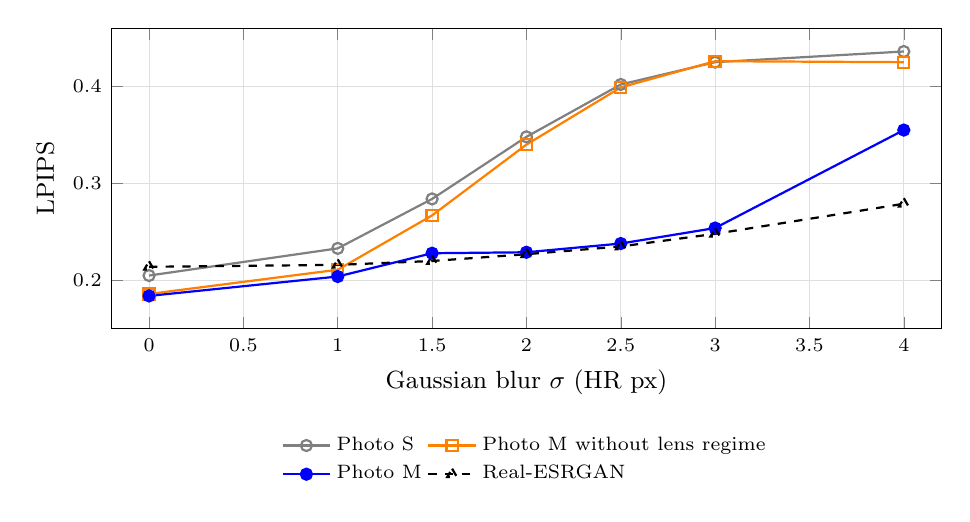
\begin{tikzpicture}
\begin{axis}[width=\columnwidth,height=5.4cm,xlabel={Gaussian blur $\sigma$ (HR px)},ylabel={LPIPS},
  xmin=-0.2,xmax=4.2,ymin=0.15,ymax=0.46,grid=major,grid style={gray!25},
  legend style={font=\scriptsize,draw=none,fill=none,at={(0.5,-0.32)},anchor=north,legend columns=2,
  cells={anchor=west}},tick label style={font=\scriptsize},label style={font=\small}]
\addplot[thick,gray,mark=o] coordinates {(0,0.205)(1,0.233)(1.5,0.284)(2,0.348)(2.5,0.402)(3,0.425)(4,0.436)};
\addlegendentry{Photo S}
\addplot[thick,orange,mark=square] coordinates {(0,0.186)(1,0.211)(1.5,0.267)(2,0.340)(2.5,0.399)(3,0.426)(4,0.425)};
\addlegendentry{Photo M without lens regime}
\addplot[thick,blue,mark=*] coordinates {(0,0.184)(1,0.204)(1.5,0.228)(2,0.229)(2.5,0.238)(3,0.254)(4,0.355)};
\addlegendentry{Photo M}
\addplot[thick,black,dashed,mark=triangle] coordinates {(0,0.214)(1,0.216)(1.5,0.220)(2,0.227)(2.5,0.235)(3,0.248)(4,0.279)};
\addlegendentry{Real-ESRGAN}
\end{axis}
\end{tikzpicture}
\caption{LPIPS against known blur (50 sharp 512\,px crops, blur, area downscale, upscale). With noise $4/255$ on top of
$\sigma=2$, Photo M reaches only 0.354 against Real-ESRGAN's 0.241.}
\label{fig:e3}
\end{figure}

Table~\ref{tab:lens} shows the lens-regime runs, each against a network of the same size without it. At 64$\times$8
the plain regime (run 1) mainly helps RealSR. A heavier tail with noise up to 16/255, JPEG down to quality 40, and a
second blur (run 3) moves the gain to DRealSR and gives most of the RealSR gain back. These three things changed
together, so I cannot say which one did it. Raising only the noise ceiling to 8/255 (run 4) made LPIPS on synthetic
blur with noise better (0.374 against 0.413), but A-FINE on the camera sets slightly worse than run 1 ($+0.57$,
$+0.30$). At 96$\times$12 the regime gave $-5.07$ and $-4.31$ on RealSR in two seeds. The difference between the two
seeds, 0.76, is the size of a typical decision margin in this project, which is why I replicate. On DRealSR, Photo M
gains on Sony ($-2.98$) and loses on Panasonic, Canon, and IMG ($+1.44$, $+1.35$, $+0.42$).

\begin{table}[t]
\centering
\caption{The lens-regime runs, A-FINE differences with 95\,\% bootstrap intervals. Negative is better.}
\label{tab:lens}\footnotesize
\setlength{\tabcolsep}{3pt}
\begin{tabular}{>{\raggedright}p{2.7cm}rr}
\toprule
Run, against & RealSR & DRealSR \\
\midrule
\multicolumn{3}{l}{\emph{64$\times$8, against Photo S (no lens regime)}} \\
1: lens regime & $-4.64$ [$-5.35$, $-3.96$] & $-1.30$ [$-1.92$, $-0.65$] \\
3: lens regime, heavy noise, JPEG, and blur tail & $-1.80$ [$-2.12$, $-1.48$] & $-3.44$ [$-4.08$, $-2.84$] \\
4: lens regime, noise ceiling 8/255 & $-4.06$ [$-4.68$, $-3.48$] & $-1.00$ [$-1.60$, $-0.38$] \\
\midrule
\multicolumn{3}{l}{\emph{96$\times$12, against the same network without it}} \\
2: lens regime (released as Photo M) & $-5.07$ [$-5.88$, $-4.29$] & $-0.53$ [$-1.35$, $+0.28$] \\
2, second seed & $-4.31$ [$-5.04$, $-3.62$] & $-0.26$ [$-1.06$, $+0.54$] \\
\bottomrule
\end{tabular}
\end{table}

\subsection{Speed}
On an M1 Pro with Core ML and 256\,px tiles, Photo S takes 188\,ms and Photo M 485\,ms per input megapixel on the Neural
Engine. On the GPU, Photo M takes 909\,ms, so the Neural Engine is about 1.9 times faster for it. Photo S matches the speed
of the SPAN model it is meant to replace (2.24M parameters, 189\,ms).

\section{Frame-by-Frame Video}

LocalSR upscales video frame by frame by default. I wanted to know how much the files flicker, whether a cheap filter
helps, and whether a fine-tune can make the model itself calmer.

\subsection{Test}
The clips are made from 30 still photos, 12 frames each, from 512\,px windows of a 520\,px crop. Each frame is
blurred (sigma 1.0), downscaled, and gets its own noise draw. There are five conditions: still shots with noise 2,
noise 4, and noise 2 plus JPEG 75, and shake (a random shift of 0 to 3 HR pixels per frame, up to $3/4$ of an LR
pixel), clean and with noise 2. So the correct output is known exactly. Flicker is the per-pixel standard deviation of
luma (0 to 255) over the 12 frames after the known shifts are undone. The ground truth scores 0. Sharpness is LPIPS on
frames 0 and 6.

\subsection{The Files Flicker}
Photo S flickers 2.42 on a still shot with noise 2 and 4.01 under shake with noise, against 1.30 and 2.51 for its L1
parent. Over the five conditions Photo S flickers 1.5 to 1.9 times as much as the L1 parent, and its detail band 1.9 to
3.2 times as much. I read this as the GAN texture following the noise of each frame. Photo M (2.45, 4.20) behaves like
Photo S. Real-ESRGAN flickers less on noisy still shots without JPEG, because it removes more noise, and more than Photo S
on the JPEG still shots (3.28) and under shake (4.50 clean).

\subsection{A Temporal Blend}
LocalSR's existing filter is a 3-frame median, applied where the output changes by at most 12 levels. It cuts Photo S's
flicker by 9 to 22\,\% on the still shots. A recursive 50\,\% blend with the previous output wherever the \emph{input}
is still, with the still mask computed on the small input frames, cuts 35 to 41\,\% (42\,\% with looser thresholds).
LPIPS gets better on the noise-only still shots and slightly worse with JPEG. In a NumPy benchmark on random frames it
costs a twelfth of the median, and the cost in the app is not measured. Under clean shake neither filter helps, and the
blend costs $+0.008$ LPIPS there. Under shake with noise both cut a little flicker (6 to 8\,\%) and improve LPIPS.

\subsection{A Consistency Fine-Tune}
I fine-tuned Photo S's GAN checkpoint for 20k updates on frame pairs: the same crop twice, each with its own noise and
a known shift of up to 3 HR pixels, with an extra loss $\lambda\,\lVert \mathrm{shift}^{-1}(f(x_1)) - f(x_2)\rVert_1$
on the overlap. The arms are released in the GAN-only form, Photo S in its head-blended form, so the cleanest comparison
is between the arms. A control arm with $\lambda=0$, trained on the same data, flickers more than Photo S (+8 to
+19\,\%), so the calming in the other arms comes from the term itself. With $\lambda=1$ the model is slightly calmer
and slightly sharper than Photo S ($-5$ to $-11$\,\% flicker). With $\lambda=4$ it removes 37 to 39\,\% of the flicker in
the four gated conditions (33\,\% with JPEG) and loses 0.034 to 0.056 LPIPS per frame. Weight blends between the
$\lambda=4$ arm and its parent lie between the two (Fig.~\ref{fig:video}). The cost per percent of flicker depends on
the condition: 0.0012 to 0.0015 LPIPS under shake, about 0.0004 on still shots with noise 4.

The rule I wrote before training asked for at least 25\,\% less flicker in four conditions, at most $+0.02$ LPIPS per
frame in every condition, at most $+0.010$ LPIPS and $+0.005$ DISTS on the web copies at 28.4\,dB, the guards, and a
seed replicate. None of the tested settings passed the flicker and per-frame LPIPS parts together. The web-copy part
could not be measured, because the arms' blend curves do not reach 28.4\,dB. In a side-by-side eye check (two photos,
grain and a slow pan, 2$\times$ crops, labels on screen, not blind), I could not tell Photo S, $\lambda=1$, the 50\,\%
blend, and $\lambda=4$ apart. I release the $\lambda=1$ and $\lambda=4$ files as experiments.

\begin{figure}[t]
\centering
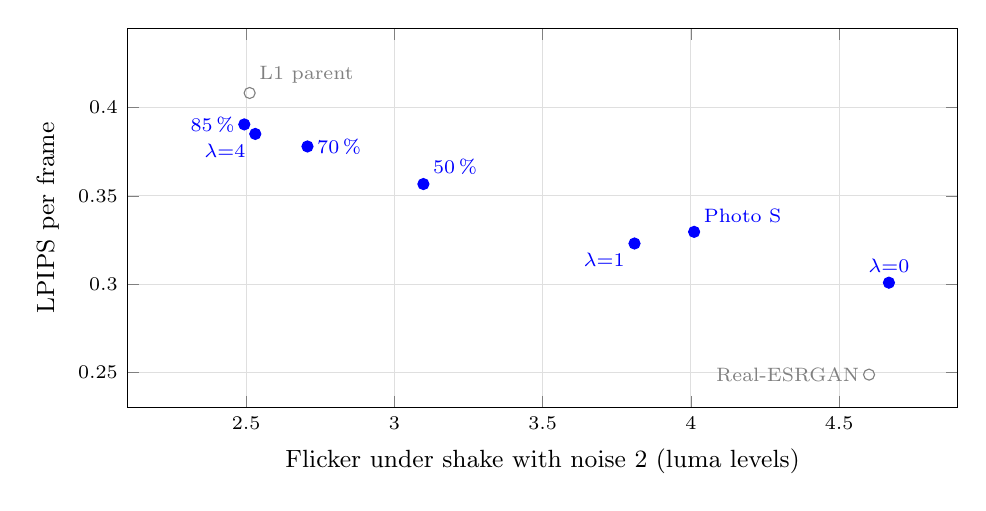
\begin{tikzpicture}
\begin{axis}[width=\columnwidth,height=6.4cm,xlabel={Flicker under shake with noise 2 (luma levels)},
  ylabel={LPIPS per frame},xmin=2.1,xmax=4.9,ymin=0.23,ymax=0.445,grid=major,grid style={gray!25},
  tick label style={font=\scriptsize},label style={font=\small}]
\addplot[only marks,mark=*,blue] coordinates {(4.011,0.3296) (3.810,0.3230) (2.531,0.3851) (4.668,0.3008)
  (3.098,0.3567) (2.707,0.3780) (2.494,0.3905)};
\addplot[only marks,mark=o,gray] coordinates {(2.512,0.4083) (4.601,0.2487)};
\node[anchor=south west,font=\scriptsize,blue] at (axis cs:4.011,0.3296) {Photo S};
\node[anchor=north east,font=\scriptsize,blue] at (axis cs:3.810,0.3230) {$\lambda{=}1$};
\node[anchor=north east,font=\scriptsize,blue] at (axis cs:2.531,0.3851) {$\lambda{=}4$};
\node[anchor=east,font=\scriptsize,blue] at (axis cs:2.494,0.3905) {85\,\%};
\node[anchor=west,font=\scriptsize,blue] at (axis cs:2.707,0.3780) {70\,\%};
\node[anchor=south west,font=\scriptsize,blue] at (axis cs:3.098,0.3567) {50\,\%};
\node[anchor=south,font=\scriptsize,blue] at (axis cs:4.668,0.3008) {$\lambda{=}0$};
\node[anchor=south west,font=\scriptsize,gray] at (axis cs:2.512,0.4083) {L1 parent};
\node[anchor=east,font=\scriptsize,gray] at (axis cs:4.601,0.2487) {Real-ESRGAN};
\end{axis}
\end{tikzpicture}
\caption{Flicker against sharpness under shake with noise 2. Photo S, its fine-tunes ($\lambda$), blends with 50, 70,
and 85\,\% of the $\lambda=4$ arm and the rest from Photo S's GAN, Photo S's L1 parent, and Real-ESRGAN. Lower left is
better.}
\label{fig:video}
\end{figure}

\section{Limitations and Negative Results}

\begin{itemize}
\item \textbf{Noisy soft input} is the clearest weakness (Fig.~\ref{fig:e3}). On DRealSR, Photo M still loses on
  Panasonic, Canon, and IMG what it gains elsewhere.
\item \textbf{The judges disagree.} A-FINE ranks Real-ESRGAN first on every set, sharp input included, and rewards
  calmer, less grainy texture. On the sealed set Real-ESRGAN also has the lowest DISTS. LPIPS and DISTS favour my
  files over the models they are meant to replace. A user study~\cite{su} warns that these distances can fail on small
  differences, and I have no rater study of my own.
\item \textbf{Video} was measured on synthetic clips from still photos, not on real footage, and the eye check was not
  blind.
\item \textbf{A bug I found:} my first controlled-blur test cropped 512\,px from 256\,px validation tiles, which gave
  128\,px crops without an error. The comparisons inside that test stayed fair, but it understated the noise weakness.
  Fig.~\ref{fig:e3} is the corrected test.
\item \textbf{Negative results:} the noise ceiling alone (run 4) did not help on the camera sets, the heavier tail (run
  3) only moved the gain between the camera sets, and the video fine-tune did not pass its rule.
\end{itemize}

\section{Conclusion}

What surprised me most is how far a small model gets with little training data: 1{,}397 source photos.

The key takeaway: I made two heavily optimised models that run in the background on the Neural Engine. On web
photos they beat or match the models they are meant to replace in LocalSR, with clearly higher fidelity. They
are not state of the art. Much larger models like Real-ESRGAN are still ahead on soft, noisy camera photos, and
by A-FINE everywhere.

The weights are released under CC BY 4.0, the network code and an upscaling script under the MIT licence.

\section*{Acknowledgements}
The network layout follows Philip Hofmann's PULSE specification, and the training data is his lucid-cc0-v2-hc
collection of CC0 photographs from pxhere.

\begin{thebibliography}{99}\footnotesize
\bibitem{realesrgan} X.~Wang, L.~Xie, C.~Dong, and Y.~Shan, ``Real-ESRGAN: Training real-world blind super-resolution
  with pure synthetic data,'' in \emph{Proc. ICCV Workshops}, 2021.
\bibitem{bsrgan} K.~Zhang, J.~Liang, L.~Van Gool, and R.~Timofte, ``Designing a practical degradation model for deep
  blind image super-resolution,'' in \emph{Proc. ICCV}, 2021.
\bibitem{span} C.~Wan \emph{et al.}, ``Swift parameter-free attention network for efficient super-resolution,'' in
  \emph{Proc. CVPR Workshops}, 2024.
\bibitem{pulse} P.~Hofmann, ``PULSE,'' \url{https://huggingface.co/Phips/PULSE}, MIT licence.
\bibitem{lucid} P.~Hofmann, ``lucid-cc0-v2-hc,'' \url{https://huggingface.co/datasets/Phips/lucid-cc0-v2-hc}, CC0.
\bibitem{mks} J.~P.~Costella, ``The magic kernel,'' \url{https://johncostella.com/magic/}.
\bibitem{msssim} Z.~Wang, E.~P.~Simoncelli, and A.~C.~Bovik, ``Multiscale structural similarity for image quality
  assessment,'' in \emph{Proc. Asilomar Conf. Signals, Systems and Computers}, 2003.
\bibitem{dinov2} M.~Oquab \emph{et al.}, ``DINOv2: Learning robust visual features without supervision,''
  \emph{TMLR}, 2024.
\bibitem{sliced} E.~Heitz, K.~Vanhoey, T.~Chambon, and L.~Belcour, ``A sliced Wasserstein loss for neural texture
  synthesis,'' in \emph{Proc. CVPR}, 2021.
\bibitem{pix2pix} P.~Isola, J.-Y.~Zhu, T.~Zhou, and A.~A.~Efros, ``Image-to-image translation with conditional
  adversarial networks,'' in \emph{Proc. CVPR}, 2017.
\bibitem{improvedgan} T.~Salimans \emph{et al.}, ``Improved techniques for training GANs,'' in \emph{Proc. NeurIPS},
  2016.
\bibitem{lpips} R.~Zhang, P.~Isola, A.~A.~Efros, E.~Shechtman, and O.~Wang, ``The unreasonable effectiveness of deep
  features as a perceptual metric,'' in \emph{Proc. CVPR}, 2018.
\bibitem{dists} K.~Ding, K.~Ma, S.~Wang, and E.~P.~Simoncelli, ``Image quality assessment: Unifying structure and
  texture similarity,'' \emph{IEEE TPAMI}, 2022.
\bibitem{afine} D.~Chen, T.~Wu, K.~Ma, and L.~Zhang, ``Toward generalized image quality assessment: Relaxing the
  perfect reference quality assumption,'' in \emph{Proc. CVPR}, pp.~12742--12752, 2025.
\bibitem{topiq} C.~Chen \emph{et al.}, ``TOPIQ: A top-down approach from semantics to distortions for image quality
  assessment,'' \emph{IEEE TIP}, 2024.
\bibitem{su} Su \emph{et al.}, ``Rethinking image evaluation in super-resolution,'' arXiv:2503.13074, 2025.
\bibitem{realsr} J.~Cai, H.~Zeng, H.~Yong, Z.~Cao, and L.~Zhang, ``Toward real-world single image super-resolution: A
  new benchmark and a new model,'' in \emph{Proc. ICCV}, 2019.
\bibitem{drealsr} P.~Wei \emph{et al.}, ``Component divide-and-conquer for real-world image super-resolution,'' in
  \emph{Proc. ECCV}, 2020.
\bibitem{stablesr} J.~Wang, Z.~Yue, S.~Zhou, K.~C.~K.~Chan, and C.~C.~Loy, ``Exploiting diffusion prior for
  real-world image super-resolution,'' \emph{IJCV}, 2024.
\bibitem{div2k} E.~Agustsson and R.~Timofte, ``NTIRE 2017 challenge on single image super-resolution: Dataset and
  study,'' in \emph{Proc. CVPR Workshops}, 2017.
\bibitem{bootstrap} B.~Efron and R.~J.~Tibshirani, \emph{An Introduction to the Bootstrap}. Chapman \& Hall, 1993.
\bibitem{lai} W.-S.~Lai \emph{et al.}, ``Learning blind video temporal consistency,'' in \emph{Proc. ECCV}, 2018.
\bibitem{tecogan} M.~Chu, Y.~Xie, J.~Mayer, L.~Leal-Taix\'e, and N.~Thuerey, ``Learning temporal coherence via
  self-supervision for GAN-based video generation,'' \emph{ACM TOG}, 2020.
\end{thebibliography}

\end{document}
